
\newpage
\section{Anhang}

\subsection{Musteranmeldeformular}
\begin{figure}[H]
    \centering
    \caption{Musteranmeldeformular von der fiktiven Person Max Müller}
    \begin{adjustbox}{height=0.85\textheight, center}
        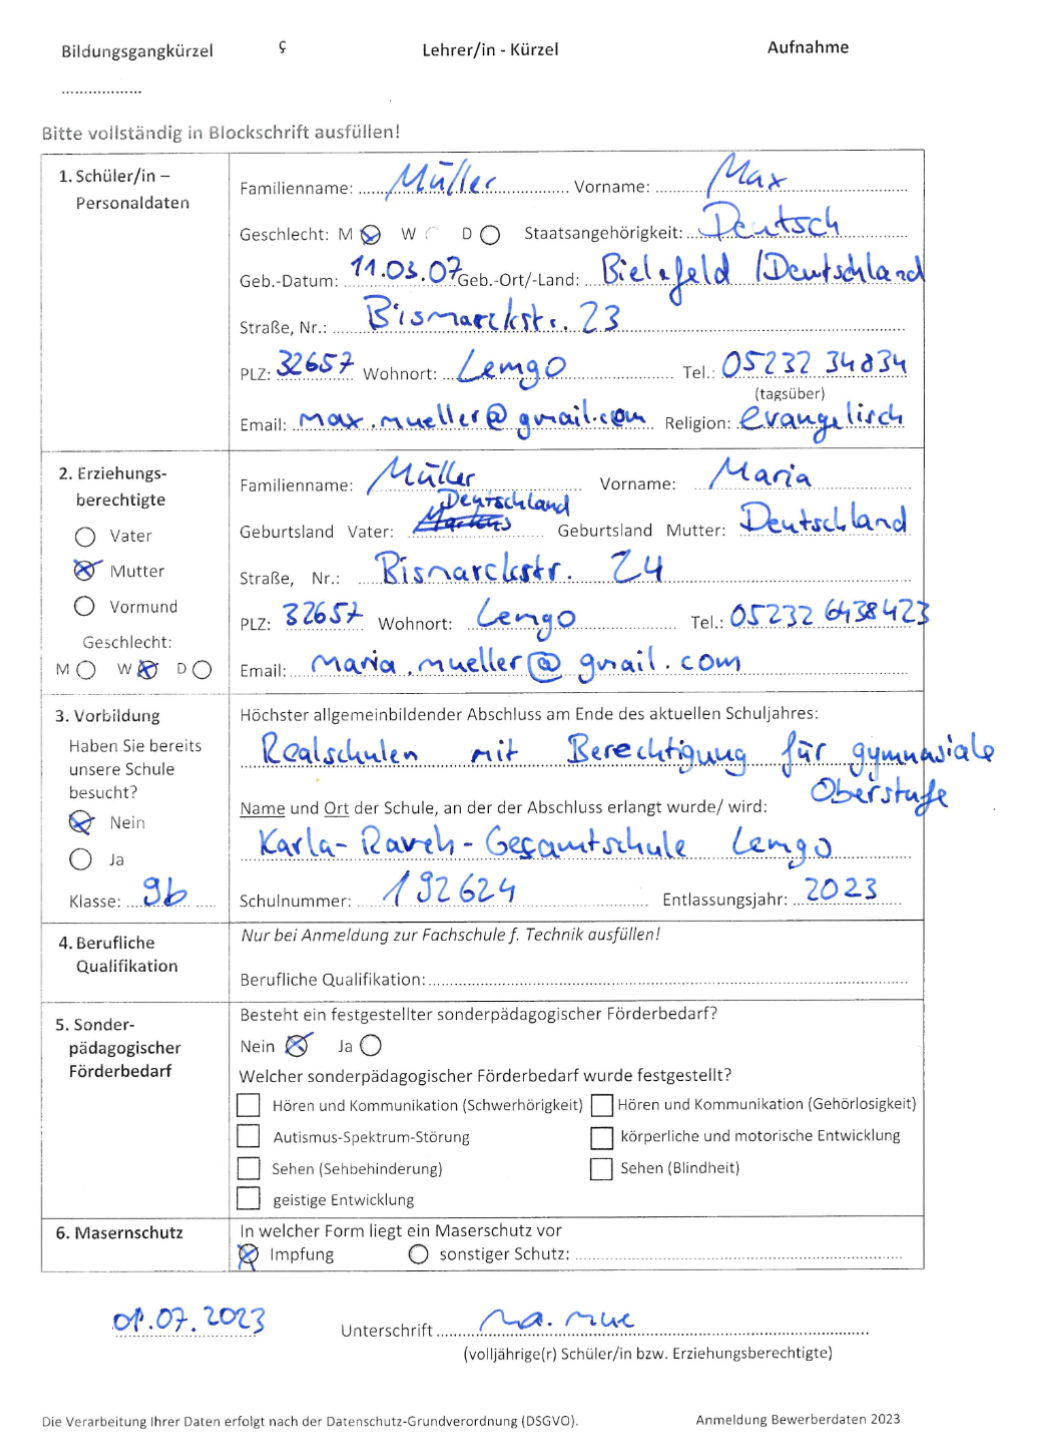
\includegraphics{bewerbungsformular1}
    \end{adjustbox}
\end{figure}

\begin{landscape}

    \begin{longtable}{p{15cm}cc}
        \caption{Your Table} \label{tab:mytable} \\
        \toprule
        Erfordernis & Beispiel & Zugehörige Ergebnisse \\
        \midrule
            Der Benutzer muss inkorrekte Daten identifizieren und korrigieren können. & a & E1, E2 \\
            Der Benutzer muss die an ihn eingereichten Formulare korrekt übertragen können. & a & E5, E6 \\
            Der Benutzer muss unzulässige Bewerbungen identifizieren können. & a & E9, E10 \\
            Der Benutzer muss die Daten datenschutzkonform in die Anwendung eintragen können und über mögliche Verstöße informiert werden. & a & E11 \\
            Der Benutzer muss erkennen können, wie er zum korrekten Prozess gelangt. & a & E12 \\
            Der Benutzer muss bezüglich Aufnahmeentscheidungen mit den Entscheidungsträgern zusammen arbeiten können. & a & E7, E8 \\
            Der Benutzer muss die Software auch bei fehlenden Daten bedienen können.  & a & \\
            Der Benutzer muss Aufnahmekriterien berücksichtigen können. & a & \\
            Der Benutzer muss Termine für Aufnahmeberatungsgespräche hinterlegen können. & a & b \\
            Der Benutzer muss Schülerakten erzeugen können. & a & b \\
            Der Benutzer muss Daten aus anderen Programmen übernehmen können. & a & b \\
            Der Benutzer muss Adressrecherchen durchführen können. & a & b \\
            Der Benutzer muss eine Kurzanleitung für den Einstieg abrufen können. & a & b \\
            Der Benutzer muss die Software auch bei fehlenden Daten bedienen können. & a & b \\
            Der Benutzer muss innerjährige Wechsel und Stufenwiederholungen erfassen können. & a & b \\
            Der Benutzer muss langfristige Beurlaubungen vermerken können. & a & b \\
            Der Benutzer muss auch komplizierte Bewerbungen und Sonderfälle bearbeiten können. & a & b \\
            Der Benutzer muss seinen bisherigen Jargon verwenden können. & a & b \\
            Der Benutzer muss die Aufgaben und Prozesse intuitiv bedienen können. & a & b \\
            Der Benutzer muss eine Adressvalidierung vornehmen können. & a & b \\
            Der Benutzer muss Erreichbarkeiten von Notfallkontakten erfassen können. & a & b \\
            Der Benutzer muss unterschiedliche Arten von Notfallkontakten erfassen können. & a & b \\
            Der Benutzer muss erkennen können, ob ein Schüler volljährig ist. & a & b \\
        \endfirsthead
        \toprule
        Erfordernis & Beispiel & Zugehörige Ergebnisse \\
        \midrule
        \endhead
        \bottomrule
        \endfoot
            Der Benutzer muss Nachweise über das Sorgerecht hinterlegen können. & a & b \\
            Der Benutzer muss Daten auch bei Dialogabbrüchen wiederherstellen können. & a & b \\
            Der Benutzer muss ähnliche Datenabfragen aus vorherigen Formularen übernehmen können. & a & b \\
            Der Benutzer muss bei Bedarf Handbücher heranziehen können. & a & b \\
            Der Benutzer muss bei Bedarf Fachterminologie nachschlagen oder verstehen können. & a & b \\
            Der Benutzer muss jederzeit darüber Bescheid wissen, welche Daten den Eltern und Schülern angezeigt werden. & a & b \\
            Der Benutzer muss den Systemstatus jederzeit einsehen können. & a & b \\
            Der Benutzer muss Bewerbungslisten in geeigneter Form exportieren können. & a & b \\
            Der Benutzer muss Daten in Schulverwaltungsprogramme wie Schild exportieren können. & a & b \\
            Der Benutzer muss Daten nach Excel exportieren können. & a & b \\
            Der Benutzer muss Berichte anfertigen können. & a & b \\
            Der Benutzer muss Anmeldezeiträume berücksichtigen. & a & b \\
            Der Benutzer muss mit anderen Behörnden zusammenarbeiten können. & a & b \\
            Der Benutzer muss über Änderungen an Bewerbungen regelmäßig informiert werden. & a & b \\
            Der Benutzer muss zusätzliche Informationen zu einer Bewerbung hinterlegen können. & a & b \\
            Der Benutzer muss Dokumente ausdrücken können. & a & b \\
            Der Benutzer muss Dokumente digitalisieren und beim Datensatz hinterlegen können. & a & b \\
    \end{longtable}




\subsection{bildungsgang}
\begin{figure}[H]
    \centering
    \caption{Testüberschrift}
    \begin{adjustbox}{width=\linewidth, center}
        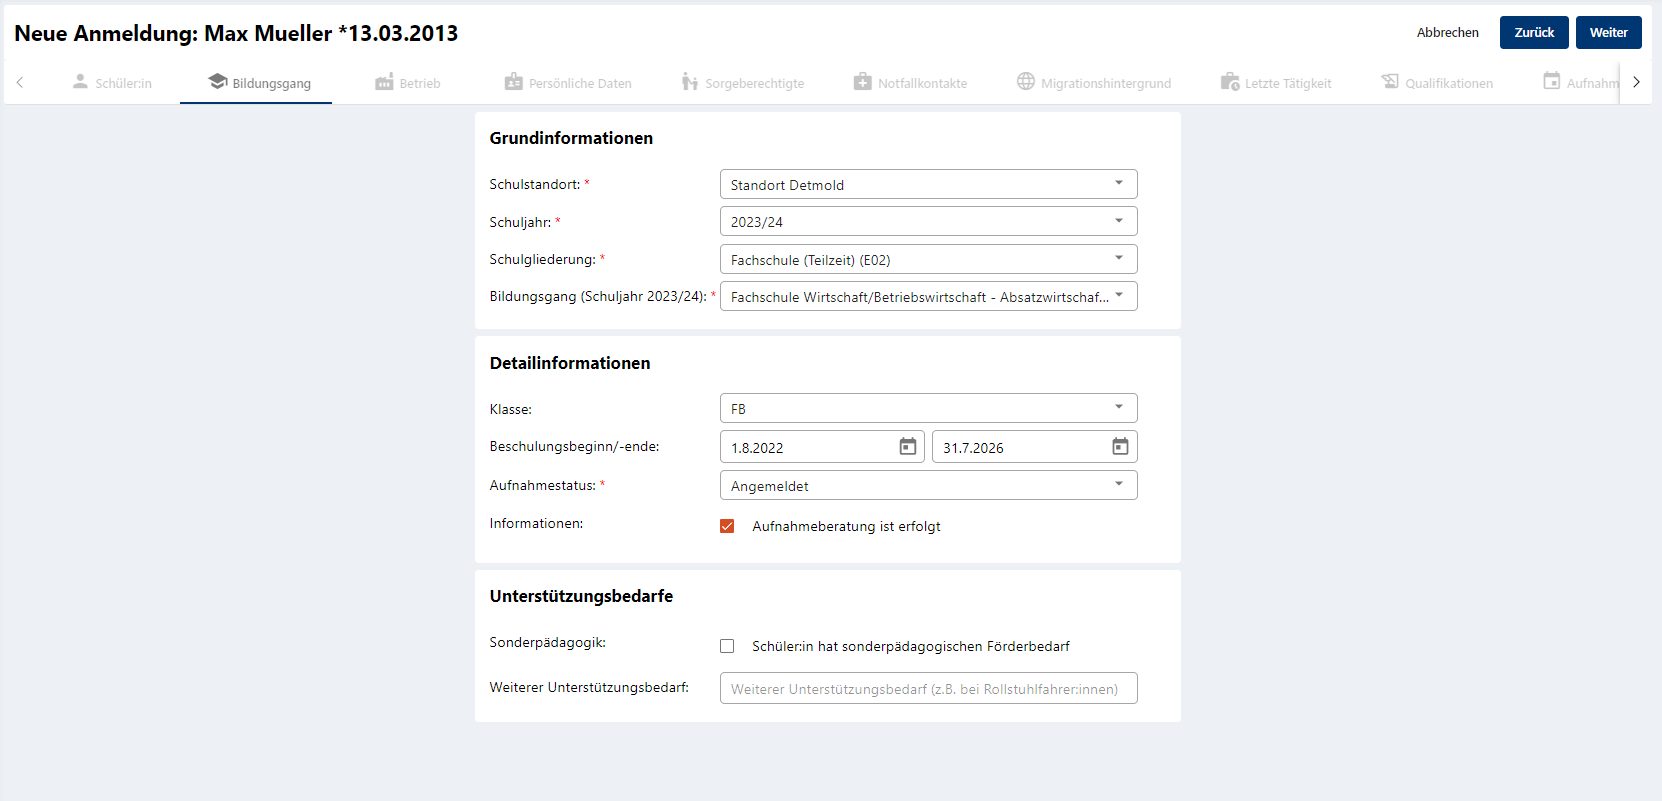
\includegraphics{bildungsgang}
    \end{adjustbox}
\end{figure}

\subsection{sorgeberechtigte-liste}
\begin{figure}[H]
    \centering
    \caption{Testüberschrift}
    \begin{adjustbox}{width=\linewidth, center}
        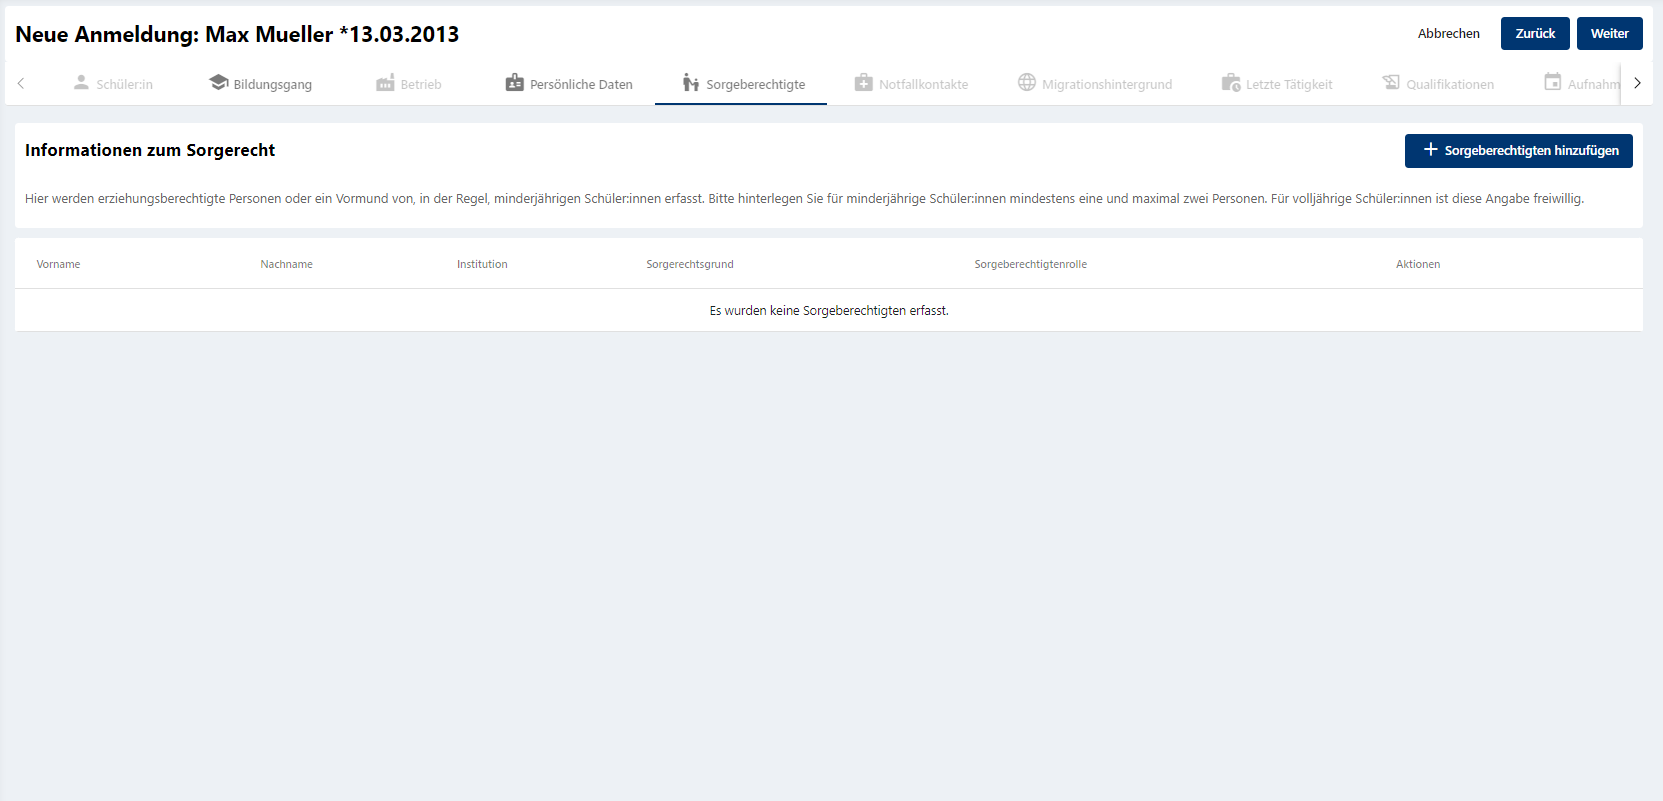
\includegraphics{sorgeberechtigte-liste}
    \end{adjustbox}
\end{figure}

\subsection{sorgeberechtigter-person}
\begin{figure}[H]
    \centering
    \caption{Testüberschrift}
    \begin{adjustbox}{width=0.5\linewidth, center}
        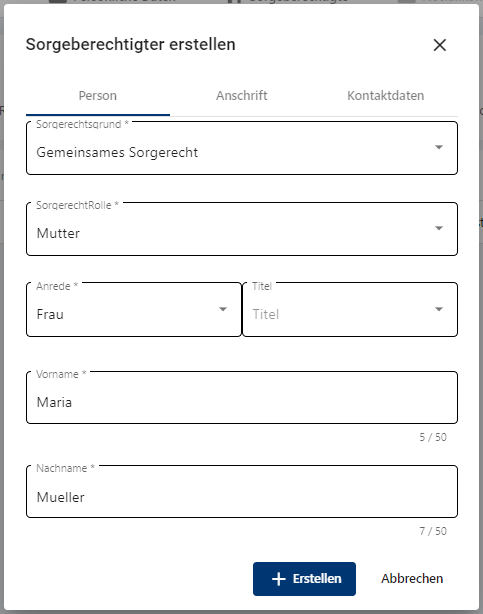
\includegraphics{sorgeberechtigter-person}
    \end{adjustbox}
\end{figure}

\subsection{sorgeberechtigter-anschrift}
\begin{figure}[H]
    \centering
    \caption{Testüberschrift}
    \begin{adjustbox}{width=0.85\linewidth, center}
        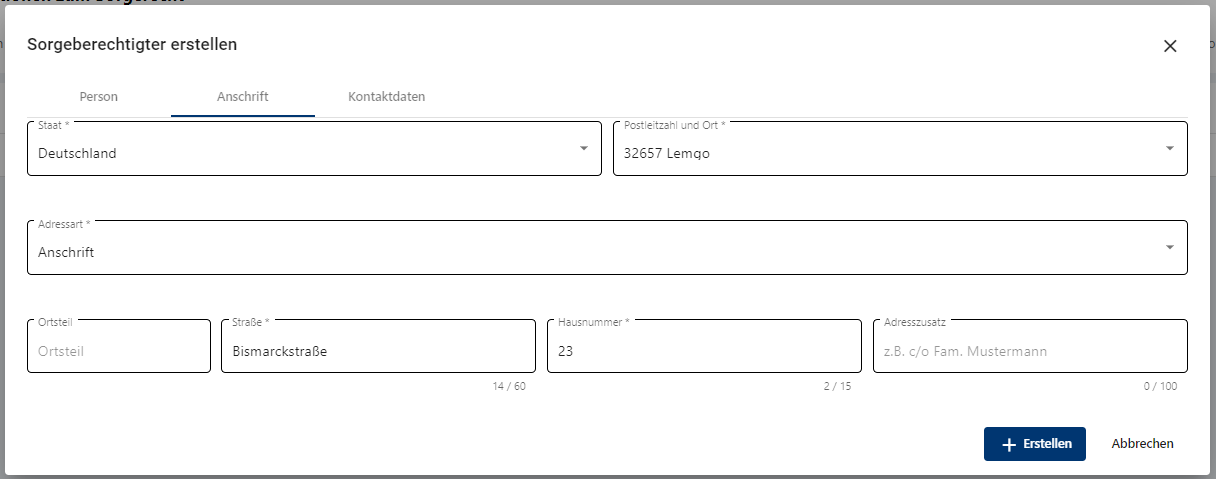
\includegraphics{sorgeberechtigter-anschrift}
    \end{adjustbox}
\end{figure}

\subsection{sorgeberechtigter-kontakt}
\begin{figure}[H]
    \centering
    \caption{Testüberschrift}
    \begin{adjustbox}{width=0.6\linewidth, center}
        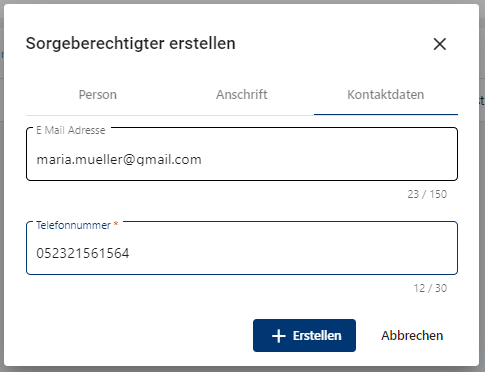
\includegraphics{sorgeberechtigter-kontakt}
    \end{adjustbox}
\end{figure}

\subsection{notfallkontakt-daten}
\begin{figure}[H]
    \centering
    \caption{Testüberschrift}
    \begin{adjustbox}{width=0.6\linewidth, center}
        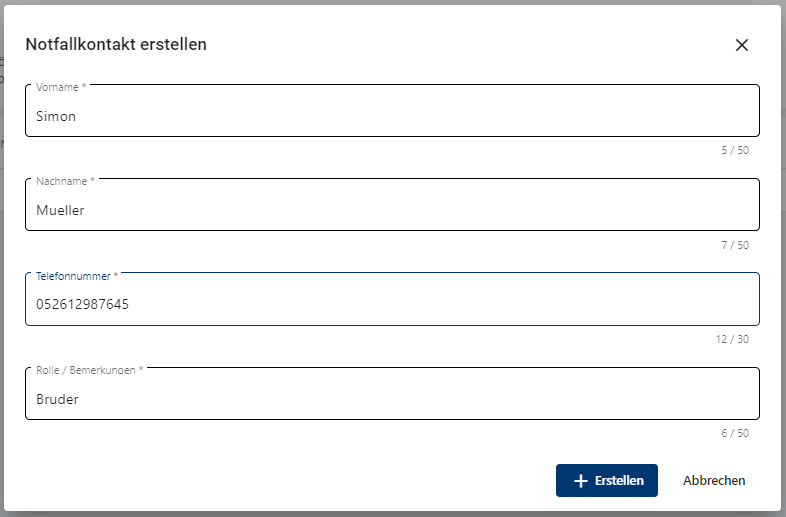
\includegraphics{notfallkontakt-daten}
    \end{adjustbox}
\end{figure}

\subsection{notfallkontakt-liste}
\begin{figure}[H]
    \centering
    \caption{Testüberschrift}
    \begin{adjustbox}{width=\linewidth, center}
        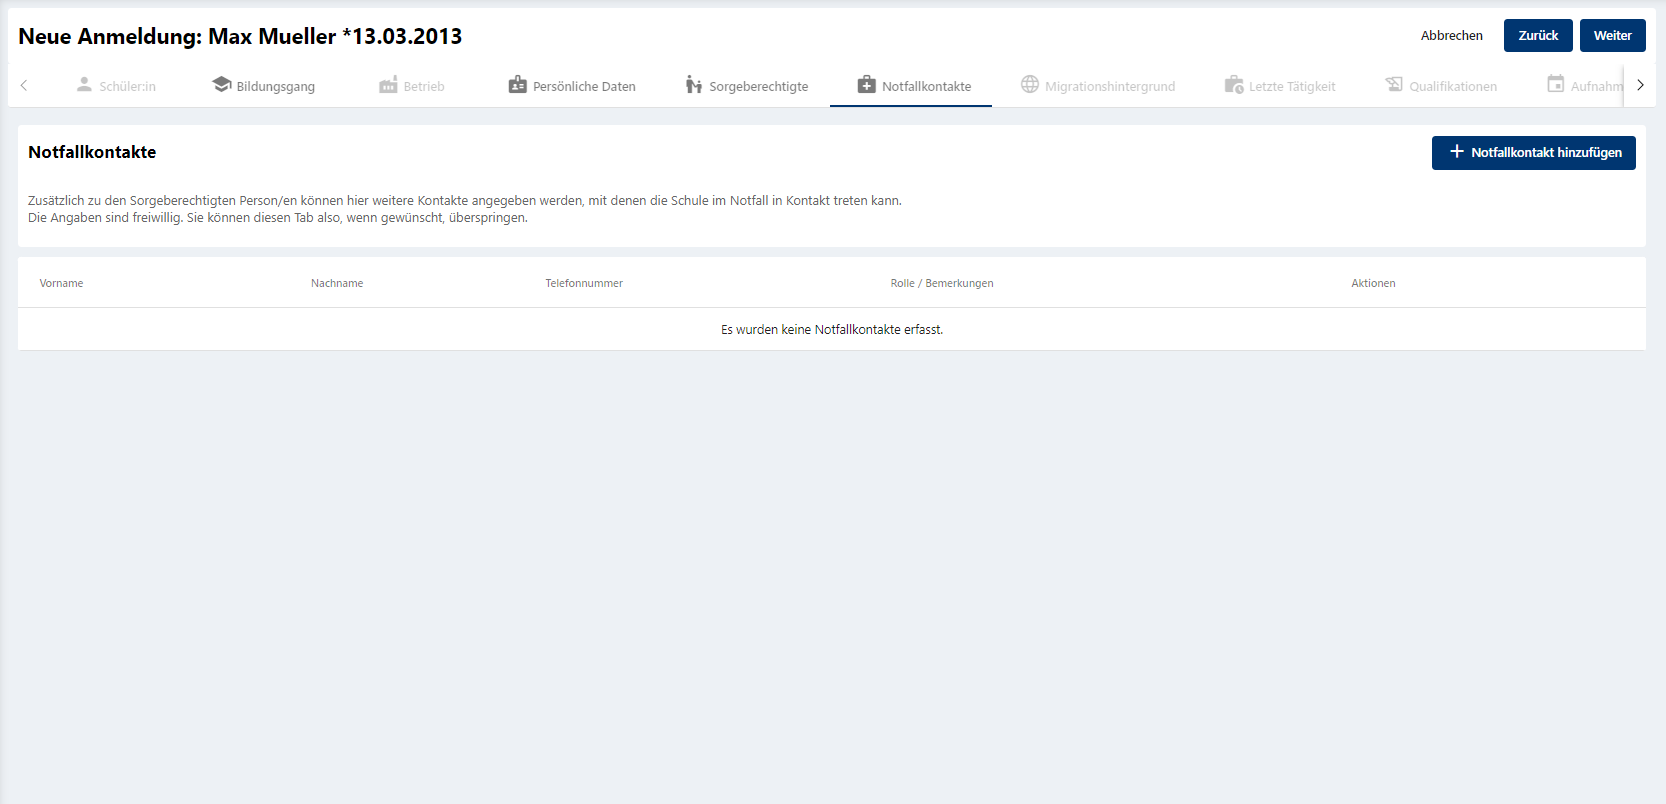
\includegraphics{notfallkontakt-liste}
    \end{adjustbox}
\end{figure}

\subsection{migrationshintergrund-liegtvor}
\begin{figure}[H]
    \centering
    \caption{Testüberschrift}
    \begin{adjustbox}{width=\linewidth, center}
        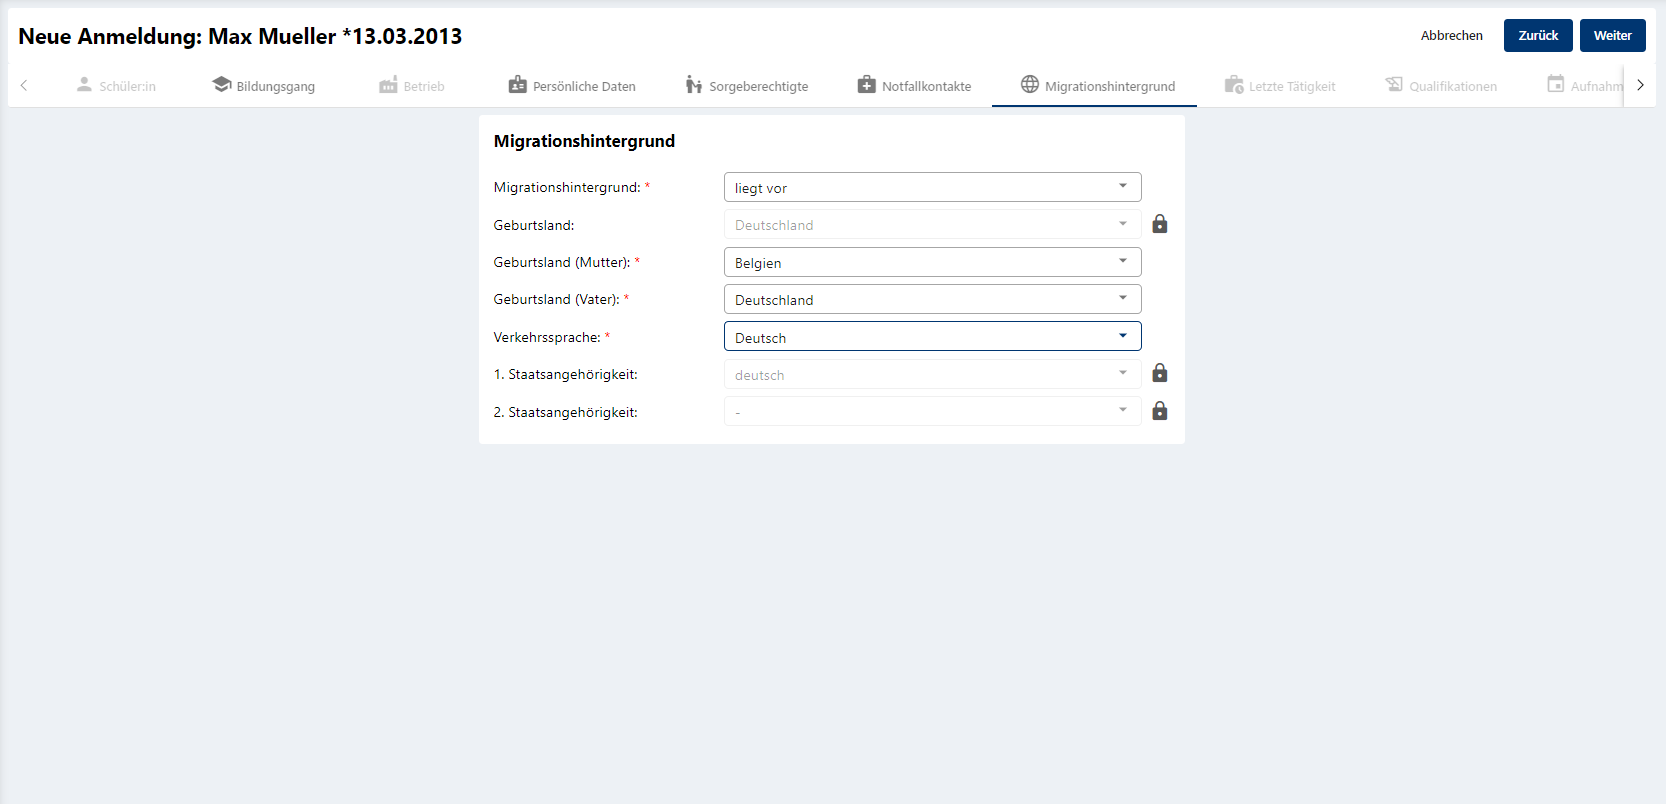
\includegraphics{migrationshintergrund-liegtvor}
    \end{adjustbox}
\end{figure}

\subsection{migrationshintergrund-liegtnichtvor}
\begin{figure}[H]
    \centering
    \caption{Testüberschrift}
    \begin{adjustbox}{width=\linewidth, center}
        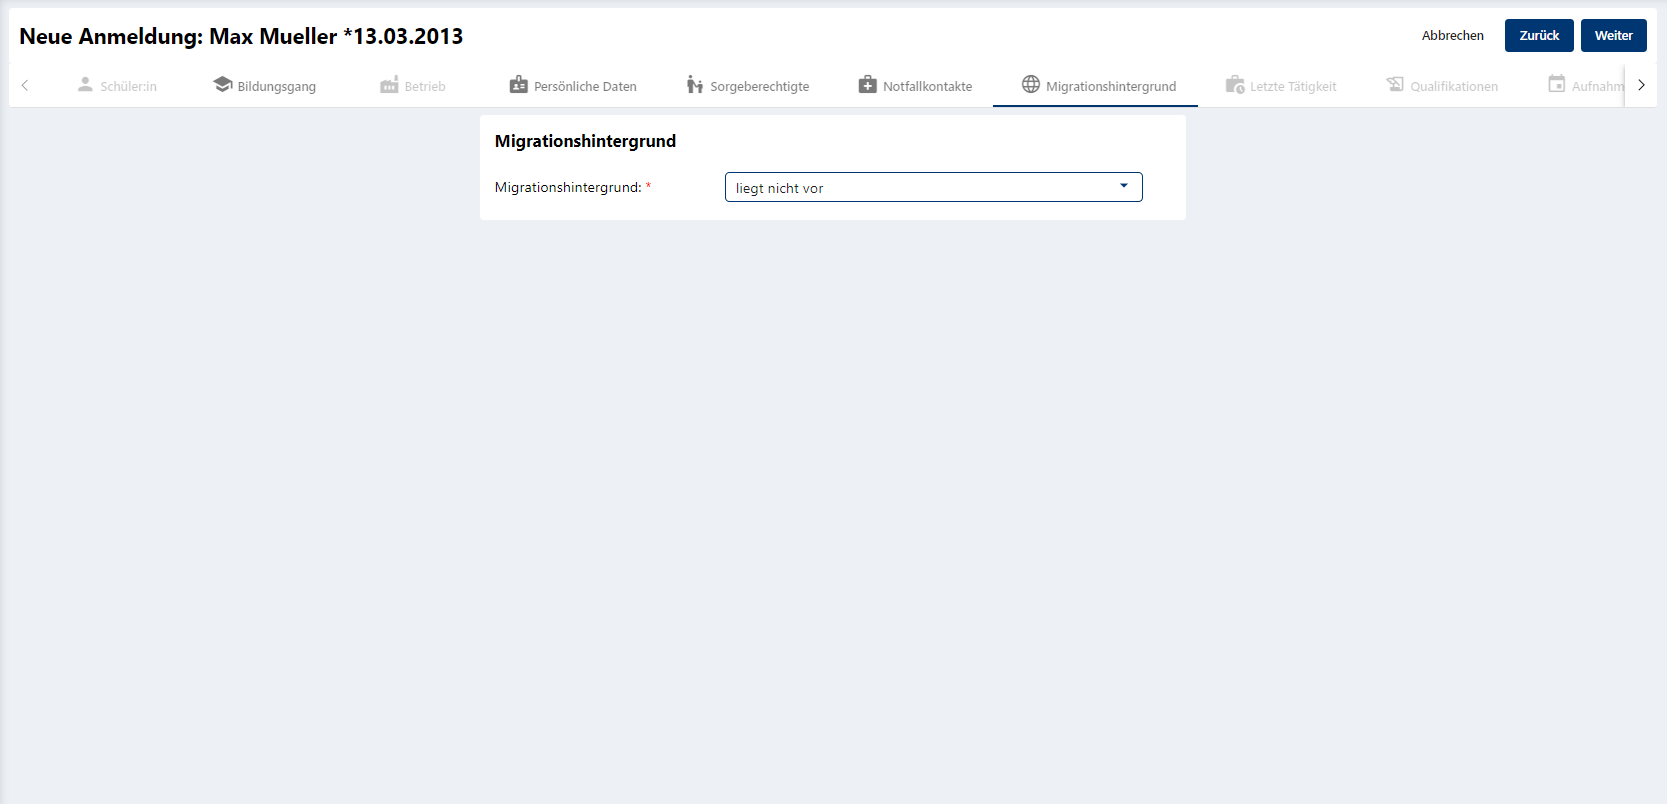
\includegraphics{migrationshintergrund-liegtnichtvor}
    \end{adjustbox}
\end{figure}

\subsection{qualifikation}
\begin{figure}[H]
    \centering
    \caption{Testüberschrift}
    \begin{adjustbox}{width=\linewidth, center}
        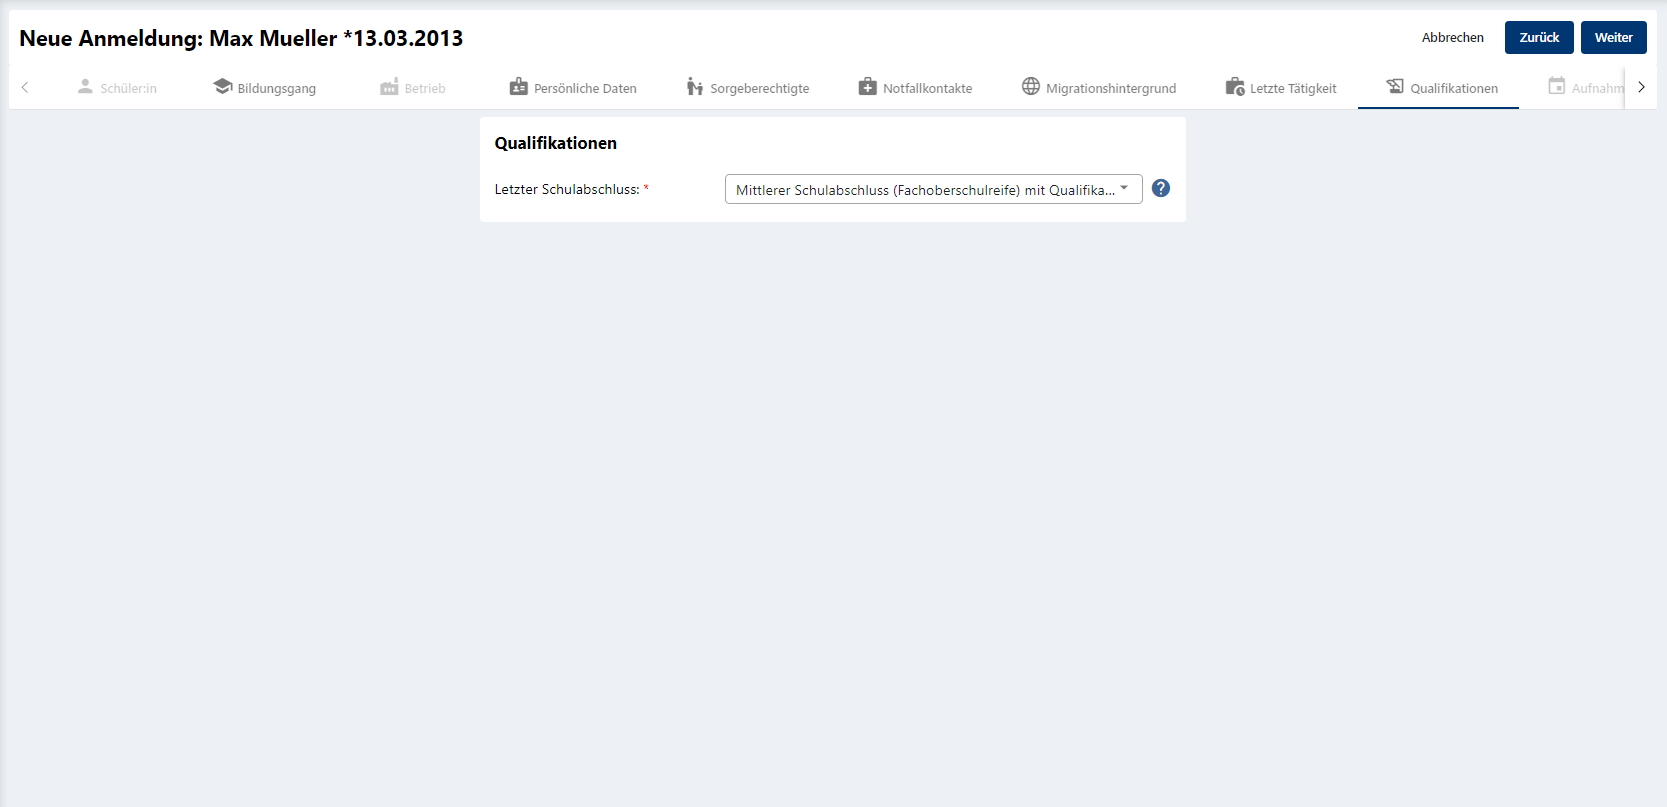
\includegraphics{qualifikation}
    \end{adjustbox}
\end{figure}

\subsection{letztetaetigkeit}
\begin{figure}[H]
    \centering
    \caption{Testüberschrift}
    \begin{adjustbox}{width=\linewidth, center}
        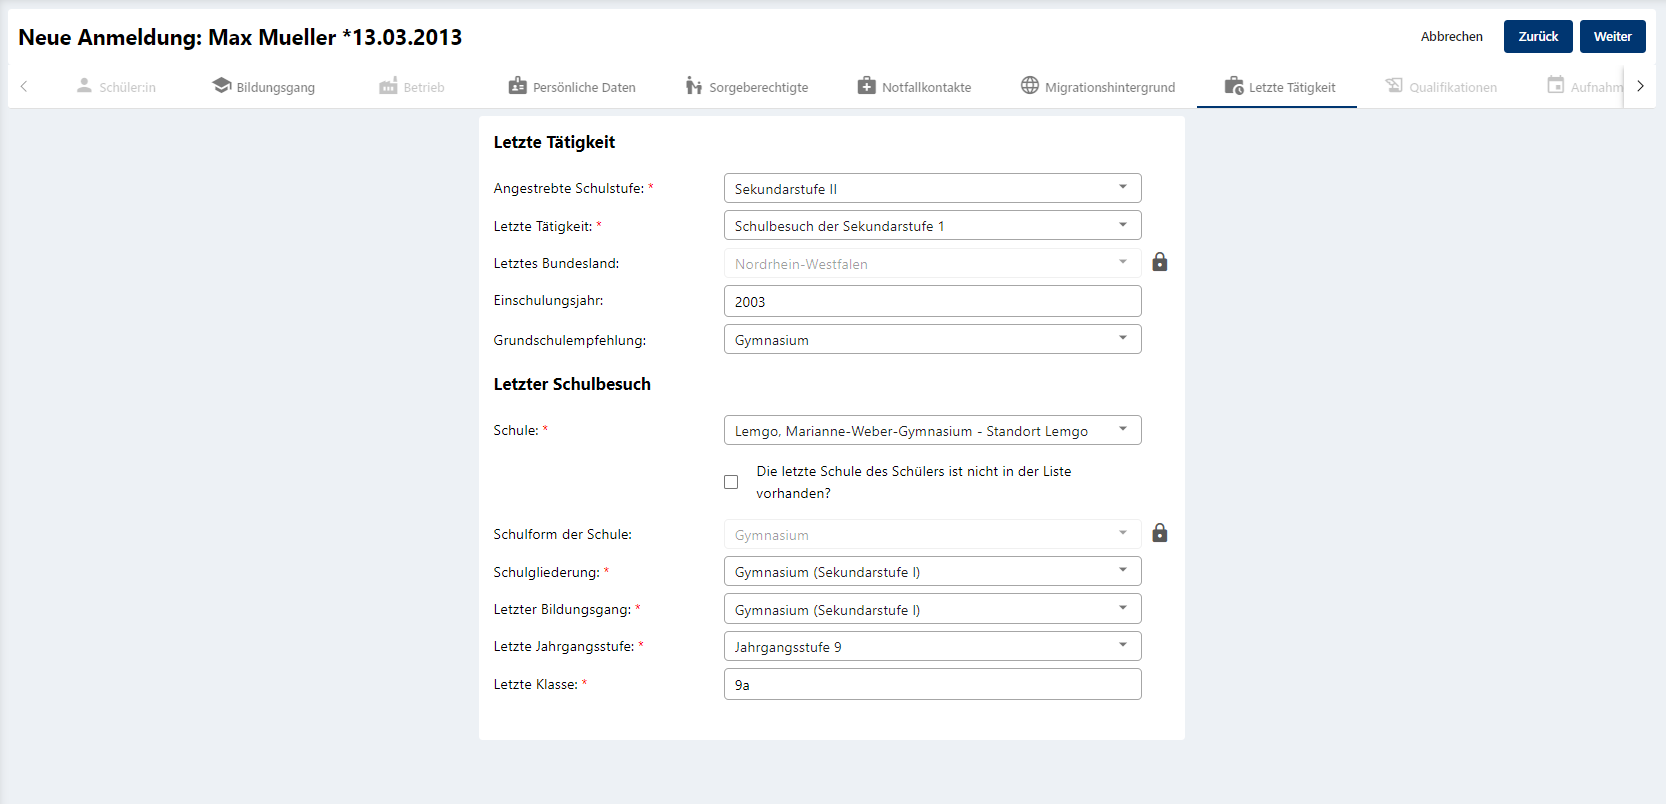
\includegraphics{letztetaetigkeit}
    \end{adjustbox}
\end{figure}

\subsection{aufnahmeberatung}
\begin{figure}[H]
    \centering
    \caption{Testüberschrift}
    \begin{adjustbox}{width=\linewidth, center}
        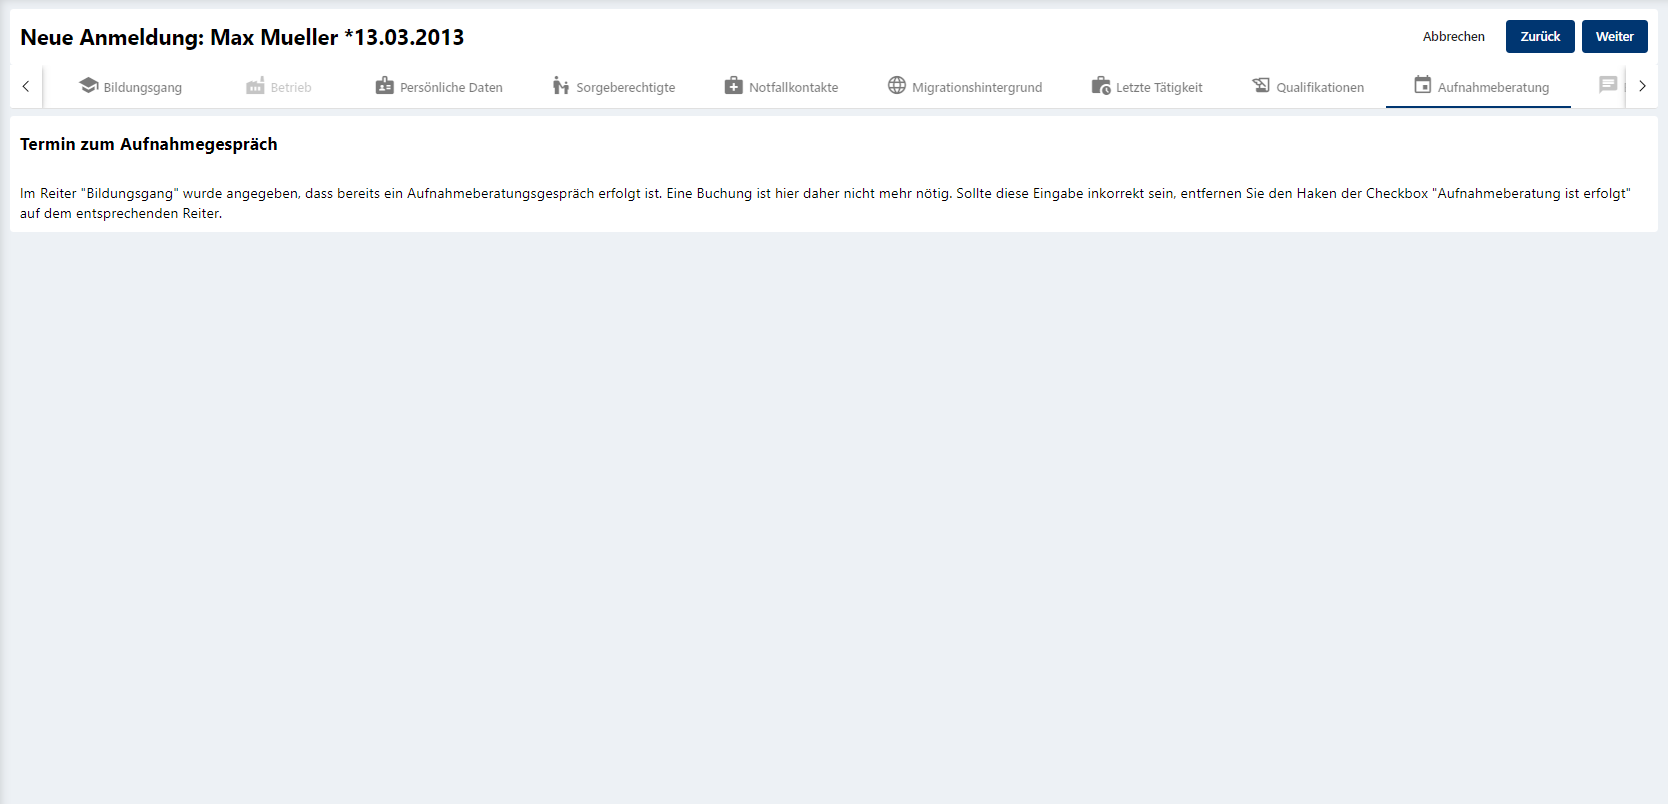
\includegraphics{aufnahmeberatung}
    \end{adjustbox}
\end{figure}

\subsection{bemerkungen}
\begin{figure}[H]
    \centering
    \caption{Testüberschrift}
    \begin{adjustbox}{width=\linewidth, center}
        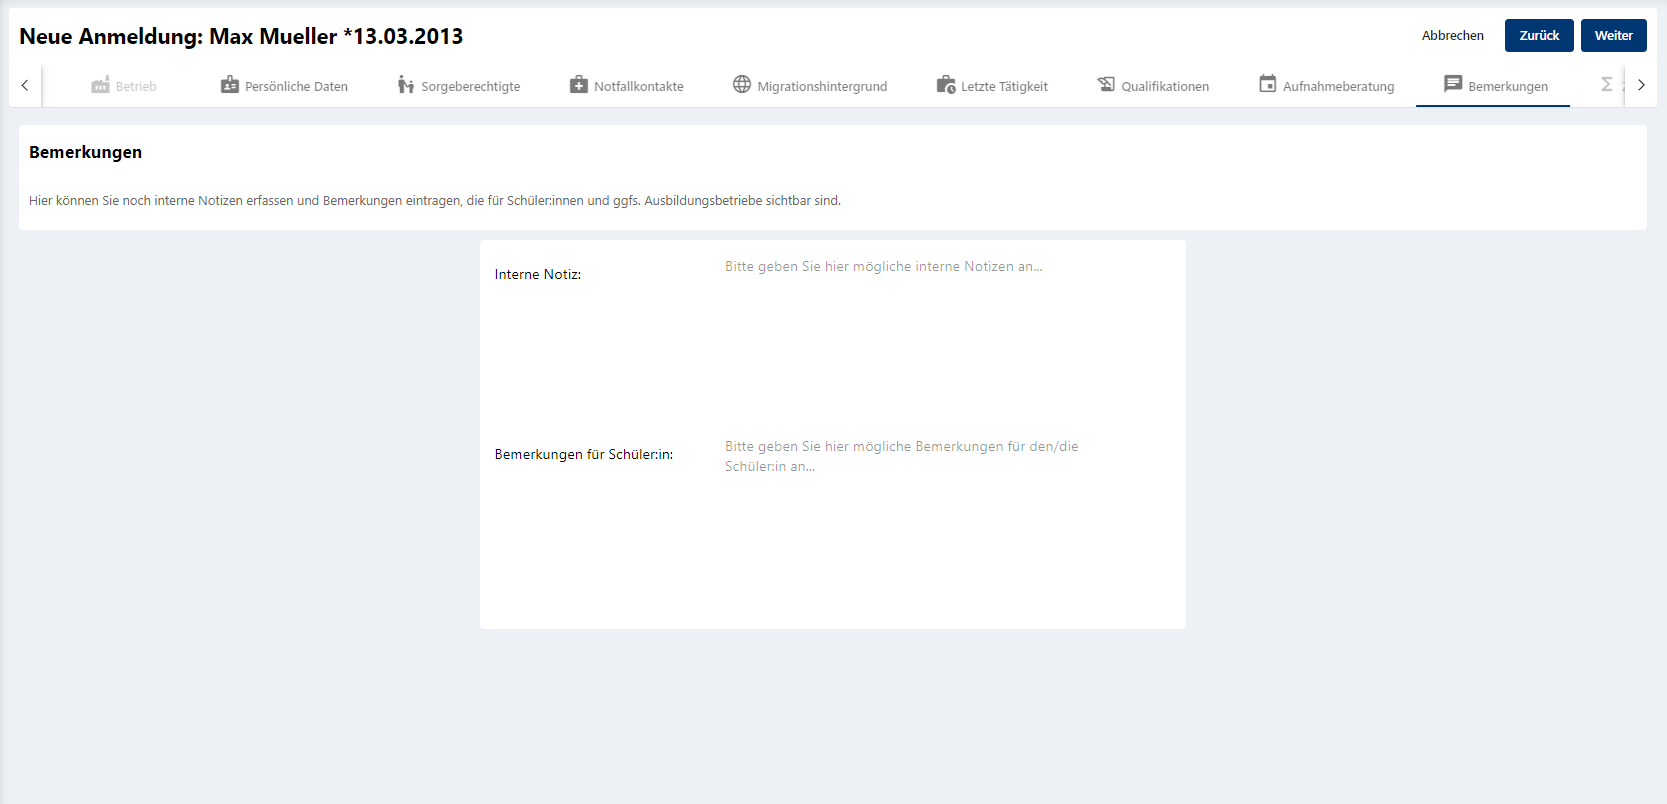
\includegraphics{bemerkungen}
    \end{adjustbox}
\end{figure}

\subsection{zusammenfassung}
\begin{figure}[H]
    \centering
    \caption{Testüberschrift}
    \begin{adjustbox}{width=\linewidth, center}
        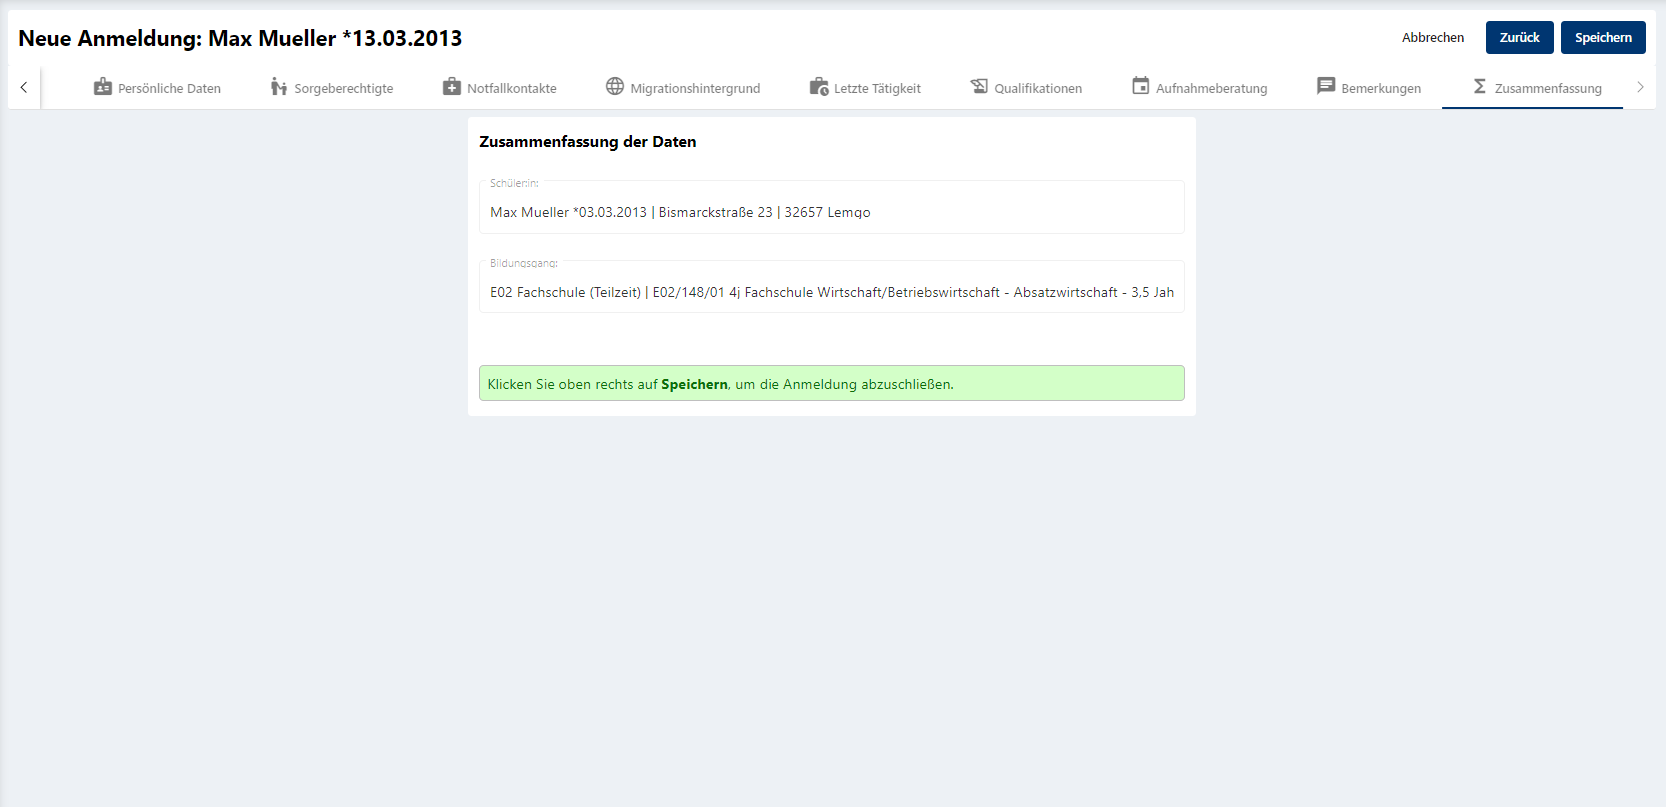
\includegraphics{zusammenfassung}
    \end{adjustbox}
\end{figure}

\subsection{bestaetigung}
\begin{figure}[H]
    \centering
    \caption{Testüberschrift}
    \begin{adjustbox}{width=\linewidth, center}
        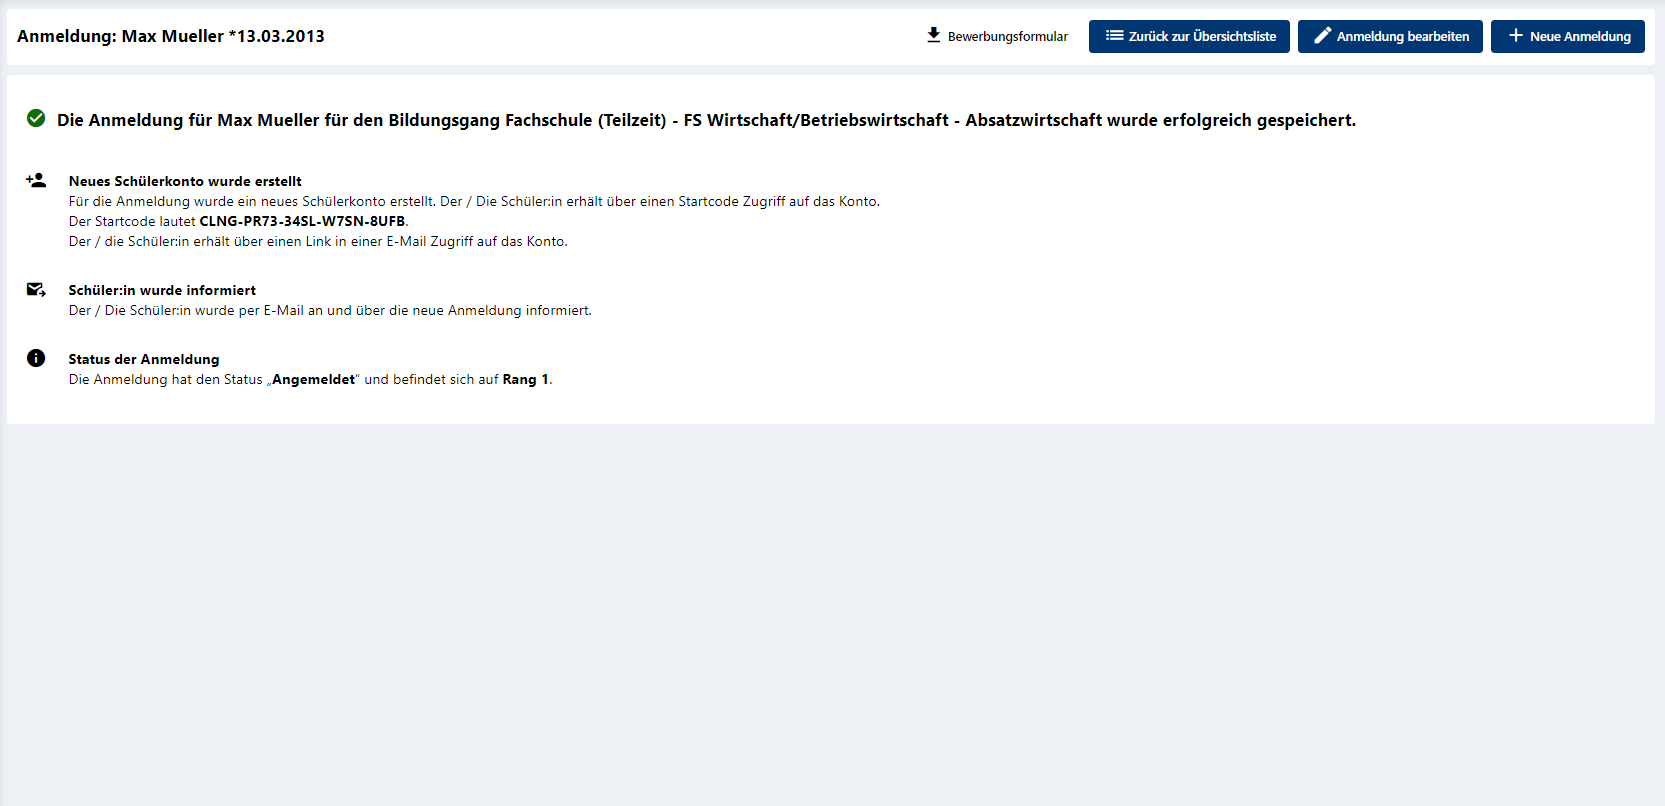
\includegraphics{bestaetigung}
    \end{adjustbox}
\end{figure}

\subsection{update-bewerbung}
\begin{figure}[H]
    \centering
    \caption{Testüberschrift}
    \begin{adjustbox}{width=\linewidth, center}
        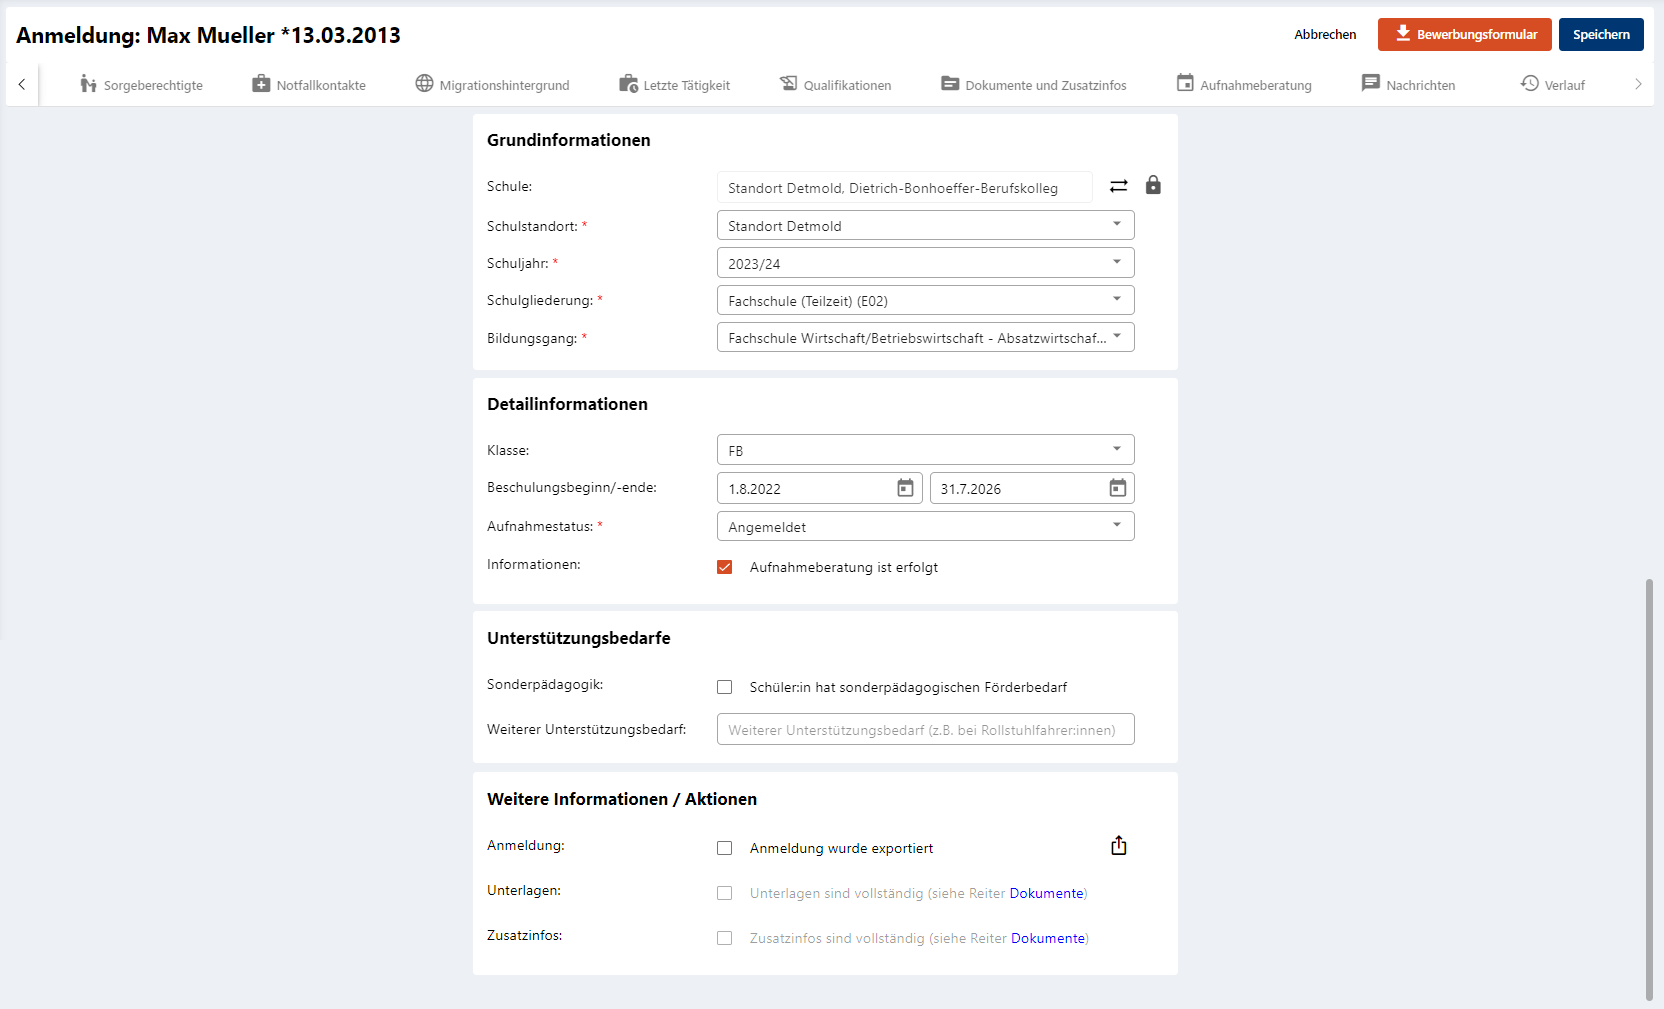
\includegraphics{update-bewerbung}
    \end{adjustbox}
\end{figure}

\end{landscape}
